\documentclass[11pt,border=5pt]{standalone}
\usepackage{fontspec}
\setmainfont{cmunrm.otf}[BoldFont=cmunbx.otf,ItalicFont=cmunti.otf,BoldItalicFont=cmunbi.otf]
\usepackage{amsmath}
\usepackage{unicode-math}
\setmathfont{NewCMMath-Regular.otf}
\usepackage{tikz}
\usetikzlibrary{arrows.meta,patterns,angles,quotes}
\begin{document}
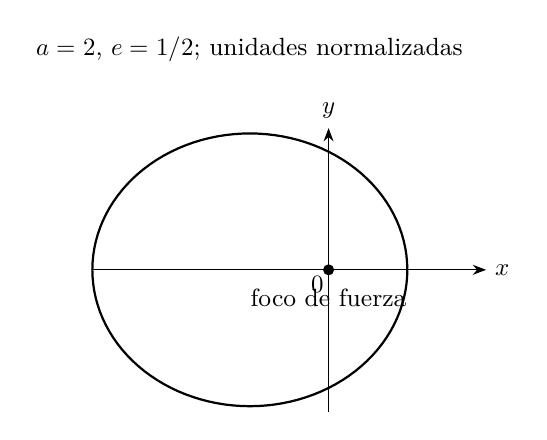
\begin{tikzpicture}[>=Stealth,font=\small,line cap=round,line join=round]
\draw[->,thin] (-3,0) -- (2,0) node[pos=1,right] {$x$};
\draw[->,thin] (0,-1.8) -- (0,1.8) node[pos=1,above] {$y$};
\node at (-0.14,-0.18) {$0$};
\draw[thick] plot coordinates {(1.00000,0.00000) (0.99726,0.09065) (0.98904,0.18105) (0.97538,0.27095) (0.95630,0.36011) (0.93185,0.44829) (0.90211,0.53523) (0.86716,0.62071) (0.82709,0.70449) (0.78201,0.78633) (0.73205,0.86603) (0.67734,0.94334) (0.61803,1.01807) (0.55429,1.09001) (0.48629,1.15897) (0.41421,1.22474) (0.33826,1.28716) (0.25864,1.34606) (0.17557,1.40126) (0.08928,1.45262) (0.00000,1.50000) (-0.09202,1.54327) (-0.18653,1.58231) (-0.28326,1.61701) (-0.38197,1.64728) (-0.48236,1.67303) (-0.58418,1.69420) (-0.68713,1.71073) (-0.79094,1.72256) (-0.89533,1.72968) (-1.00000,1.73205) (-1.10467,1.72968) (-1.20906,1.72256) (-1.31287,1.71073) (-1.41582,1.69420) (-1.51764,1.67303) (-1.61803,1.64728) (-1.71674,1.61701) (-1.81347,1.58231) (-1.90798,1.54327) (-2.00000,1.50000) (-2.08928,1.45262) (-2.17557,1.40126) (-2.25864,1.34606) (-2.33826,1.28716) (-2.41421,1.22474) (-2.48629,1.15897) (-2.55429,1.09001) (-2.61803,1.01807) (-2.67734,0.94334) (-2.73205,0.86603) (-2.78201,0.78633) (-2.82709,0.70449) (-2.86716,0.62071) (-2.90211,0.53523) (-2.93185,0.44829) (-2.95630,0.36011) (-2.97538,0.27095) (-2.98904,0.18105) (-2.99726,0.09065) (-3.00000,0.00000) (-2.99726,-0.09065) (-2.98904,-0.18105) (-2.97538,-0.27095) (-2.95630,-0.36011) (-2.93185,-0.44829) (-2.90211,-0.53523) (-2.86716,-0.62071) (-2.82709,-0.70449) (-2.78201,-0.78633) (-2.73205,-0.86603) (-2.67734,-0.94334) (-2.61803,-1.01807) (-2.55429,-1.09001) (-2.48629,-1.15897) (-2.41421,-1.22474) (-2.33826,-1.28716) (-2.25864,-1.34606) (-2.17557,-1.40126) (-2.08928,-1.45262) (-2.00000,-1.50000) (-1.90798,-1.54327) (-1.81347,-1.58231) (-1.71674,-1.61701) (-1.61803,-1.64728) (-1.51764,-1.67303) (-1.41582,-1.69420) (-1.31287,-1.71073) (-1.20906,-1.72256) (-1.10467,-1.72968) (-1.00000,-1.73205) (-0.89533,-1.72968) (-0.79094,-1.72256) (-0.68713,-1.71073) (-0.58418,-1.69420) (-0.48236,-1.67303) (-0.38197,-1.64728) (-0.28326,-1.61701) (-0.18653,-1.58231) (-0.09202,-1.54327) (0.00000,-1.50000) (0.08928,-1.45262) (0.17557,-1.40126) (0.25864,-1.34606) (0.33826,-1.28716) (0.41421,-1.22474) (0.48629,-1.15897) (0.55429,-1.09001) (0.61803,-1.01807) (0.67734,-0.94334) (0.73205,-0.86603) (0.78201,-0.78633) (0.82709,-0.70449) (0.86716,-0.62071) (0.90211,-0.53523) (0.93185,-0.44829) (0.95630,-0.36011) (0.97538,-0.27095) (0.98904,-0.18105) (0.99726,-0.09065) (1.00000,-0.00000)};
\fill (0,0) circle (2pt);
\node at (0,-0.35) {foco de fuerza};
\node at (-1,2.8) {$a=2$, $e=1/2$; unidades normalizadas};

\end{tikzpicture}
\end{document}
